\chapter{Related Work}
This chapter will describe what work has been done within treatment of depression related to digital phenotyping and context generation. Secondly, a series of previous contributions will be presented which deal with computing mobility features including how these features can be used in a medical context. Thirdly, a brief insight into exisiting mobile sensing frameworks will be given, including how the \textit{Mobility Features Package} will fit into one of these frameworks. Lastly, an example of a recommender system is given for which the \textit{Mobility Features Package} is an ideal use case.

% \section{Depression in Context}
% \subsection{Major Depressive Disorder}
Major depression MDD is a commonly occurring, seriously impairing, and often recurrent mental disorder. The World Health Organization ranks major depressive disorder as the 4th leading cause of disability worldwide \cite{murray1996} and projects that by 2020 it will be the second leading cause due to currently unexplained increasing prevalence in recent cohorts. The illness is characterized by depressed mood, low interest in doing anything, impaired cognitive function, and low quality of sleep, and changes in appetite \cite{mdd}. The illness is twice as prevalent in women, and on average affects one in six adults during their lifetime. The causes for MDD are many, among them is a heritability of 35\% and many environmental factors such as problems during childhood, however no perfect model for explaining the disease fully currently exists. Early-onset MDD is found to lead to difficulties later in life, including low educational attainment, teen pregnancy, divorce, and unstable employment \cite{costs_of_depression}. Furthermore, MDD is also a predictor for elevated risk of onset, persistence, and severity of a wide range of physical disorders and an increased rate of early mortality as well as suicide. Although research shows that treatment can reverse many adverse effects, only a minority of people with MDD receive treatment and many who do receive treatment receive extensive-, high-quality treatment. The current treatment is to manage the illness through psychotherapy as well as medication. Given the prevalence of depression, there is a need to find effective, evidence-based, cost-effective treatments for the broader public. 

% \subsection{Treating Depression with Activity Scheduling}
Activity Scheduling is a behavioral treatment for patients suffering from depression \cite{comparative_effectiveness_psycho_treatments}. in which patients monitor their daily activities as well as their mood. The goal is for patients to learn how they can increase the number of pleasant activities and positive interactions with their environment, using their own data. Low-intensity treatments such as guided self-help look promising - especially the field of  Behavioural Activation (BA), which is a component of Cognitive-Behavioural Therapy, which has gotten an increased amount of attention. The findings were that BA can be a viable option as low intensity, guided self-help treatment for mild to moderate cases of depression \cite{behavioural_activation_for_depression}. One meta-study finds that this approach shows promise even when there is a reduced number of face to face therapy sessions or even when done remotely \cite{comparative_effectiveness_psycho_treatments}. A second meta-study also concludes that it is an attractive option for treating depression, due to its relatively uncomplicated nature as well as being resource-efficient \cite{behavioural_activation_meta_analysis}.

%\section{Major Depressive Disorder}
% Major depressive disorder (MDD) is a very serious illness characterized by depressed mood, low interest in doing anything, impaired cognitive function and low quality of sleep and changes in appetite \cite{major-depressive-disorder}. The illness is twice as prevalent in women, and on average affects one in six adults during their lifetime. The causes for MDD are many, among them is a heritability of 35\%, i.e. what would be regarded as ‘nature’. The environmental factors, i.e. ‘nurture’, include a variety of abuses during childhood, however no perfect model or mechanism currently exists, which can explain the disease fully. MDD is associated with changes to the hippo-campus, responsible for the learning and memory of the brain as well as derived effects which affect the immune system. The current treatment is to manage the illness through psychotherapy as well as medication. In severe cases of MDD treatment may include electroconvulsive therapy, where the patient is given electroshock in order to affect the brain chemistry of the patient. ECT is believed to reverse symptoms of a range of mental conditions.

% \section{The costs of depression}
% Early-onset MDD is found to lead to difficulties later in life, including low educational attainment, teen pregnancy, divorce, and unstable employment. Furthermore MDD is also a predictor for elevated risk of onset, persistence and severity of a wide range of physical disorders and increased rate of early mortality as well as suicide. Although trtials show that treatment can reverse many adverse effects, only a minority of people with MDD receive treatment, and many who do receive treatment receive an extensive-,  high quality treatment.
% Major depression is a commonly occurring, seriously impairing, and often recurrent mental disorder.1, 2 The World Health Organization ranks major depressive disorder (MDD) as the 4th leading cause of disability worldwide3 and projects that by 2020 it will be the second leading cause due to currently unexplained increasing prevalence in recent cohorts.

% \section{Projections of global mortality and burden of disease from 2002 to 2030}
Projections for 2030 using WHO’s estimates of mortality and  burden of disease for 2002. Previously a model was made in 1990 but it did not account for HIV/AIDS, and in addition the numbers were somewhat outdated. The  three leading causes of burden of disease in 2030 are projected to include HIV/AIDS, (unipolar) depressive disorders and heart disease. 

% \section{Behavioral activation treatments of depression: a meta-analysis.}
Activity Scheduling is a behavioural treatment for patients suffering from depression. The basic idea is for patients to monitor their daily activities as well as their mood, and the goal is for patients to learn from their own data, how they can increase the number of pleasant activities and positive interactions with their environment. A meta-analysis of 16 studies of 780 subjects was conducted, with the findings that activity scheduling is an effective method for treating patients suffering from depression. The conclusion is therefore that it is an attractive option for treating depression given its relatively uncomplicated nature as well as being resource-efficient. 

% \section{Comparative effectiveness of psychological treatments for depressive disorders in primary care: network meta-analysis}
A broad selection of psychological treatments have been developed and are being used in primary care, including cognitive behavioural approaches. A meta-study finds that this approach shows promise even  when there is a reduced number of face to face therapy sessions or even remotely.

% \section{Behavioural activation for depression: efficacy, effectiveness and dissemination.}
Given the prevalence of depression, there is a need to find effective, evidence-based, cost-effective treatments for the broader public. Low-intensity treatments such as guided self-help looks promising - especially the field of  Behavioural Activation, which is a component of Cognitive-Behavioural Therapy, which has gotten an increased amount of attention. The findings were that BA can be a viable option as a low intensity, guided self-help treatment for mild to moderate cases of depression.

\section{Digital phenotyping: a global tool for psychiatry}
The paper \cite{digital_phenotyping} deals with the topic of collecting and aggregating user data into a so-called digital phenotype. It is predicted that by 2050, the biggest impact in psychiatry and mental health will have been the revolution in technology- and information science. Smartphones have become ubiquitous in the past decade and there are over three billion smartphones with a data plan worldwide, each of which has computing power which surpasses supercomputers of the 1990s. In areas around the world without easy access to clean water, ownership of a smartphone and by proxy, rapid access to information has become a symbol of modernity. 

\subsection{Phenotyping and Psychiatry}
In the realm of psychiatry, a current data collection problem is the dependence on self-reporting of sleep, appetite, and emotional state, even though it is recognized that depression will impair people's ability to remain objective in assessing their own behavior and thus data is prone to be faulty \cite{digital_phenotyping}. Another current problem is how it how people suffering from mental illness tend to not seek help before it is too late. Depressive relapses are therefore also often reported with considerable delay for patients currently in treatment. 

The smartphone offers an objective form of mental-state measurement which is referred to was \textit{Digital Phenotyping}, which uses built-in sensors such as geo-location, accelerometer, and human-computer interactions (HCI) to infer the state of the patient. This makes it possible to assess people by using data in a real-time fashion, rather than in retrospect as is currently is done. Digital phenotyping could in theory fill the role of a smoke detector which provides early signs of relapse and recovery, without replacing the face-to-face consultations entirely. In addition, this also allows researchers to track patients in their own environment, rather than in a clinical environment.

\subsection{The Ethical Dimension}
However, when does measurement become surveillance? Is phenotyping by using data such as geo-location too invasive? A series of ethical issues have to be addressed before digital phenotyping can realistically hope to be employed as a tool for population health. Although, some of these issues have technical solutions, such as with tracking human-computer-interactions which is mostly related to \textit{how} the user interacts with a device, i.e. the pacing with which is typed, scrolled or how long phone calls last - rather than the content of what is provided to the device i.e. what is typed, spoken during a phone call, or the websites visited. 

% Detecting Bipolar Depression From Geographic Location Data
Various contributions The aim was to identify depressive episodes of subjects using geo-location recorded from smartphones, with respect to a broader community study of Bipolar Disorder (BPD). Data was collected over 3 months, where participants also reported their depressive symptoms using a weekly questionnaire. The findings were that there is a strong link between geographic movements and depression in BPD. 

% Personalised modelling of geographic movements in depression
Depression is a very serious and very prevalent among adults. Monitoring patients over a period of time can improve the life of the patients, and lessen the burden on the healthcare system in moderate cases of depression. An avenue which is emerging is the use of geo-location tracking to monitor patients, and to assess the mental health of the patients. A study was conducted with 130 participants, which included patients with BPD and Borderline. Features were extracted from the raw GPS data and a clustering method for stationary places is described. Finding are that god location is a marker of depression but also that handling data appropriately is essential for maximizing accuracy.

% Digital biomarkers from geolocation data in bipolar disorder and schizophrenia: a systematic review
Exploring what extent gps data has been used to study serious mental illness such as BPD and schizophrenia. Monitoring with a serious mental illness is largely done face-to-face, whereas gps-based monitoring can be done remotely and in a more continuous fashion. A meta study was reviewed, and the vast majority of papers found an association between GPS-derived markers and mood which was stronger than other signals such as accelerometer data. 
\section{Learning Significant Locations and Predicting User Movement With GPS [2002]}
The paper by \cite{learning_significant_locations} from 2002 is one of the earliest contributions to present a system which uses GPS data to infer user context, and use this context. 

\subsection{Data Collection}
For this thesis a wearable GPS receiver was used which tracked user location during four months with an accuracy of 15 meters, meaning the same physical location may have resulted in slightly different GPS coordinates from day to day. For pre-processing data some of the data was discarded by setting the sensor to only log data while the user was travelling at a speed greater than 1 mile per hour, with the average human having a walking speed of about 3 miles per hour. 

\subsection{Finding Locations}
Given a data set of GPS points, a \textit{significant place} is found by examining data and finding periods of low user-movement. The duration of the period was (somewhat arbitrarily) chosen to be 10 minutes. Due to the 15 meter accuracy of the sensor, the places may be somewhat noisy from day to day, so in order to derive the exactly locations of these places, a modified version of the K-means clustering algorithm was applied to the dataset, with a radius parameter. The optimal radius for the clustering algorithm is found by examining  the graph of the number of clusters found (K) as a function of the radius. The knee of the graph signifies the radius just before the number of locations begins to converge to the number of clusters found. This procedure effectively figures out which significant places belong to the same \textit{location} and which are outliers points which should be considered noise, i.e. they either do not belong to a location or there is too low confidence to say whether they do or not. 

\subsection{Finding Sub-locations}
Within a location, several sub-locations may exists, which are perhaps best exemplified by a university campus, as a location, having several buildings for different departments, i.e. sub-locations. To find these, all \textit{significant place} data-points belonging to a \textit{location} is given as input to previously described clustering algorithm. The optimal radius is once again found by looking at the knee on the graph and from this optimal parameter choice, the sub-locations within a given location are identified.

\subsection{Prediction}
A Markov model was set up with each state representing a Location and transitions representing real-life transitions between locations. To compute the probability of a path, or a transition between places, the relative frequency of the path was computed.


\section{Density-based Spatial Clustering of Applications with Noise (DBSCAN)}
The DBSCAN algorithm is an essential algorithm for clustering GPS data points and was published by Martin Ester, Hans-Peter Kriegel, Jörg Sander and Xiaowei Xu in 1996 \cite{density-based-1996}. The core concept of DBSCAN is to cluster location data based on a density meaure rather than a pure distance measure, such as is the case with the K-means clustering algorithm. 

\begin{figure}
    \centering
    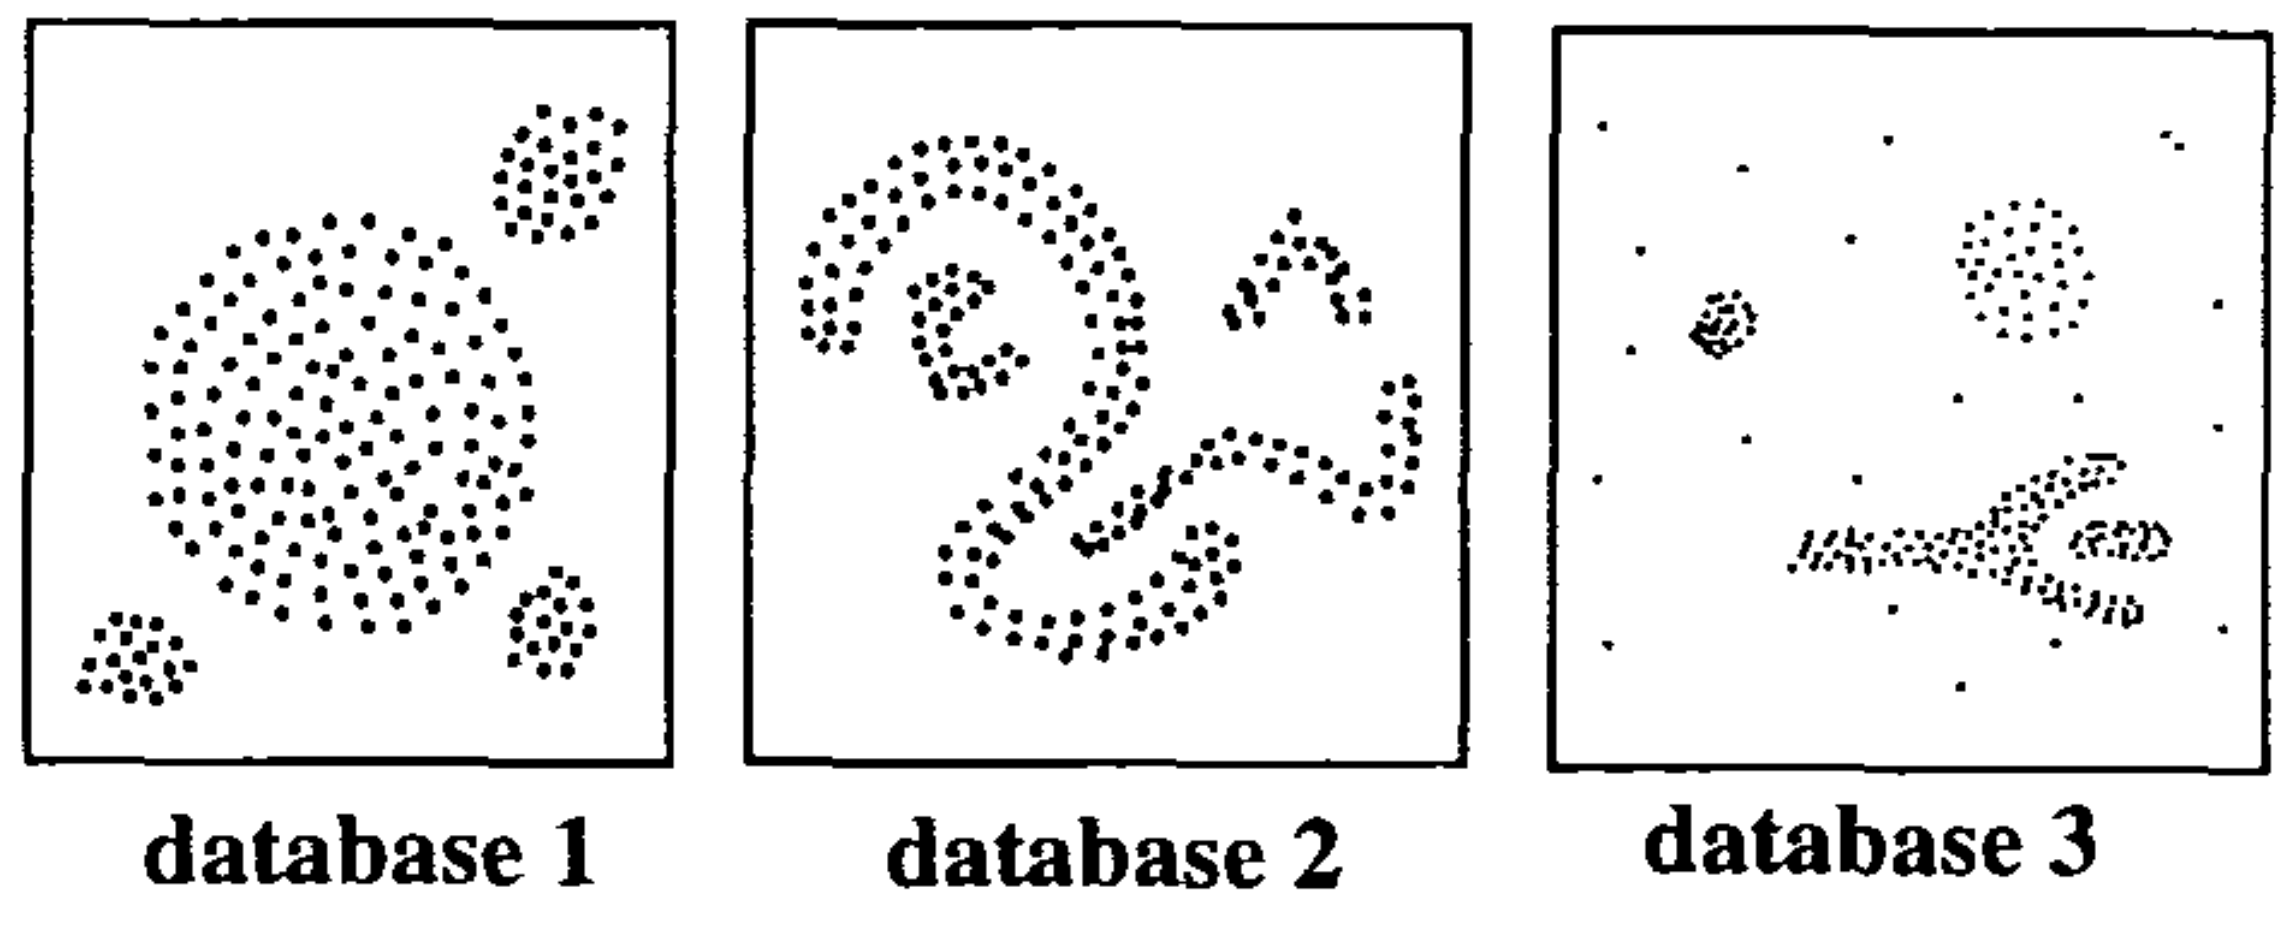
\includegraphics[width=\textwidth]{images/dbscan-clusters.png}
    \caption{Data from three different databases with very distinct cluster shapes. Database \#1 has very round clusters which would identified correctly with K-means whereas database \#2 and \#3 have clusters which would require a different clustering approach.}
    \label{fig:my_label}
\end{figure}

GPS data has a higher density inside clusters than outside the clusters and the density in noisy areas is lower than density in clusters. Here, \textit{noisy} refers to points that are spread randomly within some area and do not cluster around a centroid.

The DBSCAN algorithm will, given a set of geo-spatial data points and a small set of parameters, find these dense clusters as well as noisy data points, where the clusters correspond to places and the noisy data points are outliers which do not belong to a place. The output of the algorithm is a labelling of each point in the input dataset as either belonging to a cluster or being a noisy data point.

\section{Mathematical Definitions}

The DBSCAN paper defines a \textit{Neighbourhood} as a collection of data points within some radius, i.e. an area defined by a distance function. Within a Neighbourhood, two types of points can reside: \textit{Core points}, that is, points which are inside in the neighbourhood, and \textit{Border points } which lie on the edge of the neighbourhood and delimit it. 

\subsubsection*{Definition 1: Epsilon Neighbourhood}
An Epsilon Neighbourhood is a Neighborhood defined on a point $p$ which includes all the points $q$ which are inside a radius of $\epsilon$ of $p$, formally this is defined as $N_{\epsilon} (p) = q \in D \quad|\quad dist(p,q) \leq \epsilon$

\textit{Note: The $N_{\epsilon}$ of a border point contains much fewer points than that of a core point. }

We Require for all points $p$ and a given cluster $C$: There must be a a point $q \in C$ st. $p \in N_{\epsilon}(q)$ of and $N_{\epsilon}(q)$ contains at least $T_{min}$ points where $T_{min}$ is a parameter which defines the minimum number of points required.

\subsubsection*{Definition 2: Directly Density-Reachable (DDR)}
A point $p$ is DDR from point $q$ wrt. the parameters $\epsilon$ and $T_{min}$ if
1. $p \in N_{\epsilon}(q)$
2. $|N_{\epsilon}(q)| \geq T_{min}$ (\textit{Core Point Condition})

This implies a border point $p$ may be DDR from a core point $q$, but it is likely not true the other way around, since $N_{\epsilon}(p)$ is probably smaller than the minimum amount of points needed to satisfy the \textit{Core Point Condition}.

\subsubsection*{Definition 3: Density-Reachable (DR)}
A point $p$ is DR from a point $q$ if:
There is a chain of points $p_1, ..., p_n$ , where $p_1 = q$ and $p_n = p$, such that $p_{i+1}$ is DDR from $p_i$.
This is denoted $DR(p,q)$

\textit{Note that, only symmetric for core points, but not symmetric in general and that two border points from the same cluster may not be DR due to them not satisfying the Core Point Condition.}

\subsubsection*{Definition 4: Density-Connected (DC)}
A point $p$ is DC to $q$ if there exists a point $o$ st. both $p$ and $q$ are DR from $o$, this is denoted $DC(p,q)$. DC is a symmetric relation meaning that $DC(p,q) \iff DC(q,p)$.

\subsubsection*{Definition 5: Cluster}
A cluster is a set of DC points which is have maximal Density-Reachability. 

That is, for all points $p,q$, if $p \in C$ and $DR(p,q)$ then $q \in C$
For all points $p,q \in C$: $p$ is Density-Connected to $q$, i.e. $DC(p,q) $.

The parameters $\epsilon$ and $T_{min}$ are global, i.e. the same for all clusters.

\subsubsection*{Definition 6: Noise}
Noisy points are defined as all the points $p$ for which $p \in D \wedge p \notin C_i$ for all clusters $i = 1,...,N$, that is, all the points not belonging to any cluster.

\subsubsection*{Lemma 1}
Let $p$ be a point in $D$ for which the core point condition holds. Then, the set $O$ which is the set of DR points from $p$ (wrt. the parameters) is a cluster wrt. to the parameters. This means, a cluster $C$ contains exactly the points which are DR from an arbitrary core point of $C$.

\subsubsection*{Lemma 2}
Let $C$ be a cluster wrt. to the chosen parameters and let $p$ be a core point in $C$, then it holds that $C = O$.

\subsection{Choice of Parameters}
There is no reliable way of knowing the parameters $\epsilon$ and $T_{min}$ for each cluster in advance. Instead, the parameters are determined based on the least dense cluster, and used globally for all clusters.

\section{The DBSCAN Algorithm}
Start with a random point $p$ and get all DR points from $p$ wrt. the parameters.
Given $p \in D$: 
\begin{itemize}
\item If $p$ is a core point, then $O = DR(p)$ is a cluster (\textit{Lemma 2}).
\item Otherwise, if $p$ is a border point, then $DR(p) = \{\}$ and the algorithm proceeds to the next point $q$
\end{itemize}
Once all points have been considered, the algorithm terminates. 

Note: Since the parameters are global, the algorithm may merge two clusters according to \textit{Definition 5} if two clusters are close to each other (even if the two densities are different).

\section{The Relationship between Clinical, Momentary, and Sensor-based Assessment of Depression}
This paper by Saeb et al. published in 2015 \cite{Saeb2015} forms the basis for the context generation of this thesis, with regards how one may derive mobility features from GPS data with the features \textit{Location Entropy} and \textit{Circadian Movement} being new contributions at the time at which the paper was written. In addition, this paper also shows how certain features in particular correlate strongly with a \textit{PHQ-9} questionnaire score, which is relevant in a mental health context. Since the \textit{PHQ-9} questionnaire requires manual input from the user, and the user may forget to fill out the questionnaire, the strong correlation is great news. This could imply that it is possible to automate the patient data gathering process by simply tracking the location of the patient with a high frequency, and thus get around the issue of manually gathering biweekly, subjective questionnaire data. The \textit{PHQ-9} questionnaire (see Appendix \ref{appendix:questionnaires}).

\subsection{Pre-processing of GPS Data}
The pre-processing of GPS data is split into two phases:  Firstly, each data point is labelled as either being in a stationary or transitional state, for which the time-stamp of the current, the previous and the next data point is used. By using the this time difference as well as the distance between points the average velocity is calculated. The labelling is afterwards done by using a threshold of 1 km/h; a speed lower than the threshold indicates the state is stationary and higher is a transitional point. For analysing the data further, only the stationary points are considered. Secondly, the stationary points are processed using k-means clustering to identify frequently visited places. Since the number of places, i.e. the number of clusters for the \textit{K-means} algorithm (the paramter \textit{K}) is not know beforehand, the best parameter value is found using cross-validation. Concretely the algorithm for finding \textit{K} is to increase \textit{K} until the largest cluster found has a radius of 500 meters or lower.

\subsection{Feature Computation}
After the pre-processing step, the following features can be computed:\\

\textbf{Number of Clusters}: This feature represents the total number of clusters found by the clustering algorithm.\\
\textit{'Cluster' and 'Place' may be used interchangeably when describing features. A cluster is simply the mathematical term for a collection of data points which corresponds to a place with some GPS coordinates in the real world.}\\

$$N = K$$\\

\textbf{Location Variance (LV)}: This feature measures the variability of a participant’s location data from stationary states. LV was computed as the natural logarithm of the sum of the statistical variances of the latitude and the longitude components of the location data.\\

$$LV = \log (\sigma^2_{lat} + \sigma^2_{lon} + 1) $$\\

\textbf{Location Entropy (LE)}: A measure of points of interest. High
entropy indicates that the participant spent time more uniformly across different location
clusters, while lower entropy indicates the participant spent most of the time at some
specific clusters.\\
Calculated as 

$$Entropy = - \sum_{i=1}^N p_i \cdot \log p_i$$\\

where each $i$ represents a location cluster, $N$ denotes the total number of location clusters, and $p_i$ is the percentage of time the participant spent at the location cluster $i$. \\

\textbf{Normalized LE}: Normalized entropy is calculated by dividing the cluster entropy by its maximum value, which is the logarithm of the total number of clusters. 
$$Normalized Entropy = \frac{Entropy}{\log N}$$
Normalized entropy is invariant to the number of clusters and thus solely depends on their visiting distribution. The value of normalized entropy ranges from 0 to 1, where 0 indicates the participant has spent their time at only one location, and 1 indicates that the participant has spent an equal amount of time to visit each location cluster.\\

\textbf{Home Stay}: The percentage of time the participant has been at the cluster that represents home. We define the home cluster as the cluster, which is mostly visited during the period between 12 am and 6 am.\\

\textbf{Transition Time}: Transition Time measures the percentage of time the participant has been in the transition state.\\

\textbf{Total Distance}: This feature measures the total distance the participant has traveled in the transition state.\\

\textbf{Circadian Movement}: This feature measures to what extent the changes in a
participant’s location follow a 24-hour, or circadian, rhythm. To calculate circadian movement, we obtained the distribution of the periodicity of the stationary location data and then calculated the percentage of it that falls in the 24±0.5 hour periodicity. However, the paper does not describe in great detail how this feature is implemented.\\

\subsection{Correlations with PHQ-9}
The features which correlated strongest with the \textit{PHQ-9} scores over two weeks were the following:\\

\textbf{Circadian Movement}: This features correlated negatively with the \textit{PHQ-9} score, and can be interpreted as depressed individuals tend to have less of a routine than healthy individuals. \\

\textbf{Location Variance \& Normalized Location Entropy}: These features have a similar meaning and both correlate negative with the \textit{PHQ-9} score. The takeway here is likely that visiting very different places every single day can be seen as a sign that the individual is depressed, which also correlates with the Circadian Movement, since visiting different places every day results in a low level of routine.\\

\textbf{Home Stay}: This feature had a Strong positive correlation with the \textit{PHQ-9} score, and thus the main take away from this feature is that spending a lot of time at home is an indicator of being depressed.

\subsection{Findings}
The paper finds that depressive symptoms tend to change slowly over weeks, with little day-to-day variation and thus it makes more sensor to group data on a weekly basis. This may explain why two weeks of sensor feature correlated more strongly with the \textit{PHQ-9} than either daily sensor features or EMA measures. Unlike EMA ratings, which are momentary, the \textit{PHQ-9} assessment reports symptoms over a period of two weeks. The study conducted suggests that it is possible to monitor depression passively using phone sensor data, and in particular, GPS. Most people are unwilling to answer questions repeatedly over long periods of time, while passive monitoring could improve the management of depression in populations, allowing at risk patients to be treated more quickly as symptoms emerge, or monitoring patients’ responses during treatment.
\section{Extraction of Behavioral Features from Smartphone and Wearable Data}
Published in 2019 \cite{extraction-of-behavioural-features}, this paper focuses on many channels for collecting user data, with each channel resulting in a set of features. Examples of channels are GPS data, phone usage, step count, etc. The upside of having many channels is improved accuracy since more data is available to describe the behaviour of the user, and if certain channels are inactive during certain periods of time, the other channels can cover the missing data, and thus periods of missing data will be avoided with high likelihood. 

The paper uses the \textit{AWARE Framework }\cite{aware2015} to collect data such as  \textit{Bluetooth}, \textit{Call-log}, \textit{Location}, \textit{Campus Map}, \textit{Phone Usage}, \textit{Step Count} and \textit{Sleep State} (via FitBit).

\subsection{High Level Derived Features}
The daily behaviour of the user is predicted through four high-level features extracted from the data channels.\\

\textbf{User mobility}: The movement patterns of the user are derived from location tracking and the campus map feature.\\ 

\textbf{Communication Patterns}: Derived from call log and text messages.\\

\textbf{Mobility and communication}: Derived from Bluetooth device IDs within range, i.e. Bluetooth scan.\\

\textbf{Physical activity:} Derived from step-count during different windows of the day, i.e. when the user is walking a lot.\\

\subsection{Time windows}
The day (24 hours) is split into 4 time windows, which helps identify where the home is, since the user likely sleeps the same place most days of the week, which is likely during the \textit{night} time-window.

\begin{itemize}
\item Night (00-06)
\item Morning (06-12)
\item Afternoon (12-18)
\item Evening (18-00)
\end{itemize}

\subsection{Location Features}
GPS coordinates collected throughout the day have a time stamp connected to them, which makes it possible to calculate a list of interesting features within a day of the user moving around. The features are similar to those found in \cite{Saeb2015} adds two additional features, namely \textit{Radius of gyration} and \textit{Time spent at top3 clusters}.

However a couple of additional contributions are found. Firstly a \textit{bout} is defined as a small window of time, which can be defined based on the granularity wanted, i.e. 5 minutes. 

Furthermore, a clear definition for the \textit{home} cluster is given as being everything within 10 meters of the center of the home location center. Time spent at home is defined at time spent within 100 meters of the home centroid. The activity of studying is defined as spending 30 minutes or more in an academic building, while sedentary, which is taking fewer than 10 steps per \textit{bout}.

\subsection{Bluetooth Features}
From the Bluetooth Scan, the devices found each have a unique ID and can therefore be categorized into the following groups:

\begin{itemize}
    \item Self, i.e. the user (the device scanned most often)
    \item Related, ex colleagues, flatmates (scanned less often)
    \item Other, other people (scanned least often)
\end{itemize}

The three categories are created through K-means clustering, by firstly creating two clusters ($K=2$), i.e. self and others. Secondly another model is fitted to the data with $K=3$ clusters, and the model which fits the data the best is chosen, i.e. through cross validation or BIC.


\subsection{Phone Usage}
Phone usage is based on the screen state which at any time can be only one of the following: On, off, lock, unlock. Tracking the state of the screen together with the timestamp at which the state changes, a few features can be calculated, which are:

\begin{itemize}
    \item Number of unlocks per min
    \item Time spent interacting with the phone
    \item Total time unlocked
    \item Hour of day of first unlock/turned on
    \item Hour of day of last unlock, lock, turned off
    \item Time spent interacting with phone (sum of time between unlock and off/lock)
    \item Standard deviation of time spent interacting with phone
\end{itemize}


\subsection{Sleep Features}
By tracking heart rate, and other signals with a FitBit watch, the FitBit API gives access to the \textit{sleep state} of the user, which at any time is one of the following: Asleep, restless, awake, unknown.

A number of samples will made during the night and thus the simplest features which can be created are the number of samples in each of the four states. 
From this, two higher-level features are computed, which are: \\

Weak Sleep Efficiency: $WSE = \frac{n_{asleep} + n_{restless}}{n_{asleep} + n_{restless} + n_{awake}}$\\

Strong Sleep Efficiency: $SSE = \frac{n_{asleep}}{n_{asleep} + n_{restless} + n_{awake}}$\\

With $n_{state}$ being the number of samples for that state.


\subsection{Steps Features}
From the step-count channel features pertaining to the fine-grained activity, without the location, for a whole day, can be calculated:

\begin{itemize}
    \item Number of steps
    \item Max steps in a \textit{bout}
    \item Number of active \textit{bouts}
    \item Min, Max, Avg. length of sequence active \textit{bouts} in a row
\end{itemize}
    
\subsection{Behavioural Change Tracking}
The change in the user's behaviour over a longer time perioid, i.e. a few weeks can be tracked by using a number of the proposed features, and is done by applying a simple linear regression as well as a piecewiese linear regression (with two lines) to the dataset. The calculate behavioural change features are then the following:

\begin{itemize}
    \item Derivatives ($a_i$) of the linear model: $y=a_1 x_1 + a_2 x_2 + ... + a_n x_n + c$.
    \item Change in slope (derivative) for each behavioural feature
\end{itemize}

Given data for $n \in \mathbb{Z}$ timesteps, i.e. weeks, choose some breakpoint $m < n \in \mathbb{Z}$ and create the piecewiese linear function:

\[ \begin{cases} 
      a_1 x_1 + a_2 x_2 + ... + a_n x_n + c & t <    m \\
      b_1 x_1 + b_2 x_2 + ... + b_n x_n + d & m \leq n 
   \end{cases}
\]

The two line segments are then fitted to the data with a feature selection algorithm. The resulting slope vectors for the selected features are then behavioural features.

%%%%%%%%%%%%%%%%%%%%%%%%%%%%%%%%%%%%%%%%%%%%%%%%%%%%%%%%%%%%%%%%%%%%%%


\section{Inferring Human Mobility from Sparse Low Accuracy Mobile Sensing Data}
Human Mobility is relevant for a number of different applications such \textit{disease spread,} \textit{urban planning}, \textit{managing traffic }as well as understanding \textit{social interactions}. Previous contributions within these fields have been using Call Detail Records (CDR) which is the art of triangulating the user's location by use of cell-phone towers. These sources produces very course-grained estimates wrt. location and time. For this paper a more traditional location data sampling was used, using the GPS tracker in smartphones, however, for longitudinal studies it can be a problem for the phone battery if the sampling rate is too high. Therefore a more low-energy approach is used where the sampling rate- and the location accuracy are low. 

\subsection{Data Collection and Features}
A study with 6 participants was conducted in which location data collected continuously and the users filled out an online diary on a daily basis. Given a series of temporally-ordered data points for a user, the aim was to compute features called \textit{Stops} and \textit{Places of Interest (POI)}. A \textit{POI} is defined as a location of high relevance such as that person's school, gym or a supermarket as is denoted by a type $POI = (ID, lat, lon)$ and a \textit{Stop} at a POI is defined as period of time in which the user stayed at a POI with a given ID, i.e. $Stop = (arrival, departure, ID)$. To find Stops, both a \textit{Gaussian Mixture Model} as well as the \textit{DBSCAN} algorithm were applied for clustering. To evaluate the best model, the $f_1$ score of each model was computed, and in the end, it was found that both algorithms performed similarly for each of the participants. 
\section{Trajectories of Depression: Unobtrusive Monitoring of Depressive States by means of Smartphone Mobility Traces Analysis} 

% Main idea
In this paper by Canzian et. al from 2015 \cite{Canzian2015}, it is discussed how existing systems for diagnosing depression require the user to interact with the device. These interactions can be input such as mood-state a few times a day, which can be highly subjective and error-prone. The paper addresses this issue via objective patient data, called \textit{Mobility Features}, which was collected via unobtrusive monitoring by using smart-phone location data. There was a significant correlation between these \textit{Mobility Features} and depressive moods similar to \cite{Saeb2015}. The paper also describes concrete models to \textit{predict} changes in depressive mood by using these features. The paper uses the \textit{PHQ-8} questionnaire as reference, which is the almost the same questionnaire as the \textit{PHQ-9} (see Appendix \ref{appendix:questionnaires}), except for only including the first 8 questions. While this paper describes many of the same features as \cite{Saeb2015}, it does so in a much more detailed and mathematical way, such as with the \textit{Routine Index} feature, which correspond to the \textit{Circadian Rhythm} feature in \cite{Saeb2015}.

\subsection{Features}
The feature described are as follows:\\

\textbf{Place: $p = (id, t_a, t_d, c)$}\\
A place is a cluster of geo-location points with a unique $id$ and a geographical center $c = (lat, lon)$. When the user arrives at the place it happens at $t_a$ and the user departs from the place at $t_d$. \\

\textbf{Mobility Trace: $MT(t_1, t_2) = [p_1, ...., p_n]$}\\
A mobility trace is a list of all places visited in the time interval $(t_1, t_2)$. $N(t_1, t_2) = n$ is the number of places visited and the time gap between $t_d (p_i)$ and $t_a (p_{i+1})$ is a period of movement.\\

\textbf{Total Distance: $D_T (t_1, t_2)$}\\
The total geodesic distance traveled in the time interval $(t_1, t_2)$.\\

\textbf{Max Distance: $D_M (t_1, t_2)$}\\
The maximum distance between any two places visited in the interval $(t_1, t_2)$.\\

\textbf{Radius of Gyration: $G(t1, t2)$}\\
The geographical area covered in the interval $(t_1, t_2)$\\

\textbf{Standard Deviation of Displacement: $\sigma_{dis}$}\\
The standard deviation between each displacement, i.e. distances from one point to another.\\

\textbf{Home Cluster: $H$}\\
The cluster most frequented cluster at 02:00, 06:00 and 20:30 on week-days.\\

\textbf{Max Distance from Home: $D_H(t_1, t_2)$}\\
The distance to the point the furthest away from home, during the interval $(t_1, t_2)$.\\

\textbf{Number of different places visited: $N_{dif} (t_1, t_2)$}\\
The number of different clusters found in the interval $(t_1, t_2)$.\\

\textbf{Number of different significant places visited: $N_{sig} (t_1, t_2)$}\\
The number of significant places visited in the interval $(t_1, t_2)$. The maximum number of significant places is 10.\\

\textbf{Routine Index: $R(t1, t2)$}\\
The degree to which the place-time distribution during the interval $(t_1, t_2)$ on a given day is similar to the distribution on other days, during the interval $(t_1, t_2)$.\\

\subsection{Smart Location Sampling}
In addition to concrete definitions of features, the paper also provides an algorithm for sampling location in way which saves phone battery. GPS data collection is very expensive if done with a high frequency and by using cheaper sensors to turn it off when necessary can therefore save a lot of battery. Concretely the accelerometer is used by an activity recognition algorithm to determine the user's activity state. Concretely this is done by modelling the user as being in a movement state, of which there are 3: \textit{Static (S)}, \textit{Moving (M)} and \textit{Undecided (U)}, where location tracking only takes place in the \textit{U} or \textit{M} states. \\

The definitions for the states are as follows:\\

\textbf{Static (S)}\\
The user is in the same location i.e. school/work. Never sample location data while in this state since it is unnecessary.\\

\textbf{Moving (M)}\\
The user is moving from place to place and the phone should therefore keep location tracking on, while in this state.\\

\textbf{Undecided (U)}\\
It is unknown whether the user is moving or not and moving to either state \textit{S} or \textit{M} is now impending. When this state is entered, the user's location $l_1$ is sampled, and after 5 minutes the location is sampled again, providing $l_2$. Then,  The distance $d = dist(l_1, l_2)$ is calculated and from this, the algorithm will transition to either \textit{S} or \textit{M} depending on the distance between the two locations.

The transitions are made, as follows:\\

\textbf{U $\rightarrow$ S}: If the distance $d < 250$ m.\\

\textbf{U $\rightarrow$ M}: If the distance $d \geq 250$ m.\\

\textbf{S $\rightarrow$ U}: If two consecutive activity recognition samples indicate user activity with over $50\%$ confidence.\\

\textbf{M $\rightarrow$  U}: If two consecutive samples are less than 250 m apart, or when an activity recognition sample indicates the user is still with more than 50\% confidence.\\
\section{Rohani: The MORIBUS \& MUBS Systems}
The prevalence of depression has led to the development of many mobile health-tech solutions and applications for monitoring diseases related to depression. However few of these application have focused on the treatment of depression. There is clinical evidence showing that depressive symptoms can be alleviated through Behavioural Activation which is a behaviour-focused treatment method for treating depression. D. Rohani is a postdoc at CACHET and has published and developed two systems during his PhD within the realm of Behavioural Activation which are the MORIBUS- and MUBS systems.

\subsection{The MORIBUS System}
The MORIBUS system \cite{moribus} by Rohani aims to make it easy for depressed patients to remember and register their behavior in order to increase their every-day positive outcomes. The system comes with a catalogue of 54 pre-made activities such as \textit{Get ready in the morning} and \textit{Eat breakfast} and has support for patients to add their own activities by manually inputting text and a rating. When an activity is completed, the patient registers this in the app along with a short reflection. The application   is able to provide the user with statistics and summaries of activity frequency and reflections.

\subsection{MUBS}
The MORIBUS system later evolved into the MUBS system, which once again addresses the issue of treating depression using Behavioural Action with a mobile health solution \cite{mubs-rohani}. The application uses a larger catalogue of pleasant activities and give recommended activities for perform, personalized to each user. The catalogue is database of 384 common enjoyable activities where each activity has been manually labelled by researchers with an activity level, and contains a category. The recommender model uses a Naive Bayes model with a set of features representing each feature and a corresponding label representing whether it is positive or negative for that individual user. The model is designed to recommend already-known activities as well as novel activities to the user which is in the spirit of behavioural activation. It was suggested to add additional features such as \textit{location}, \textit{local weather} and \textit{ambient noise} to a future edition of the recommender system. 

\subsection{Improving the Systems}
Both the MORIBUS- and the MUBS system relies on manual input from the user in order to learn which activities to recommend in the future. This can pose a problem, especially when running longitudinal studies since participant retention may suffer if the input process is too involved for the user. Rohani is therefore a very good example of an application developer who would benefit greatly from using an automated feature generation algorithm such as the \textit{Mobility Features package}.
\section{AWARE: Mobile Context Instrumentation Framework}
The AWARE Framework \cite{aware2015} is an open source toolkit and a reusable platform for capturing, inferring and generating context on mobile devices. Today, phones are full of sensors but constrained on resources such as compute power and especially battery, and this has to be considered when generating  context in real time using the phone battery. AWARE aims to ensure an easy way of collection contexts for the application developer, and it is demonstrated how the tool can can reduce the software development effort of researchers when building mobile tools for devleoping context-aware apps and doing so with minimal battery impact. By concealing and encapsulating the underlying implementation of sensor data-retrieval and exposing the inferred context as a higher level abstraction, AWARE shifts the focus from software development to data collection and analysis. This opens the research field to be less programming oriented. Currently AWARE is available on both iOS and Android and supports a number of data channels \footnote{\url{https://awareframework.com/sensors/}} such as the built-in sensors, as well as Application usage, SMS- and call-logs. Some of the channels are however not available on iOS due to the iOS API in general being more restrictive than that of the Android SDK.
\section{The CAMS Framework}
The CARP Mobile Sensing (CAMS) Framework\footnote{\url{https://github.com/cph-cachet/carp.sensing-flutter/wiki}} is a Flutter framework for adding digital phenotyping capabilities to a mobile-health app. CAMS is designed to collect research-quality sensor data from the many smartphone data channels such as sensors and location data, in addition to external sensors that the phone is connected to, such as wearable devices. The main focus of the framework is to allow application programmers to design and implement a custom mobile health app without having to start from scratch, with regards to the sensor integration, by enabling the programmers to add an array of mobile sensing capabilities in a flexible and simple manner. This would include, firstly, adding support for collecting health-related data channels such as \textit{ECG}, \textit{GPS}, \textit{Sleep}, \textit{Activity}, \textit{Step Count} and much more. Secondly, to format the resulting data according to standardized health data formats (like \textit{Open mHealth} schemas \footnote{\url{https://www.openmhealth.org/documentation/#/schema-docs/schema-library}}. Thirdly, to upload the collected data to a specific server, using a specific API (such as \textit{REST}), in a specific format, such that it may be used for data analysis. To include as many data channels as possible the application should also be able to support different wearable devices for ECG monitoring and activity tracking. Hence, the focus is on software engineering support in terms of a solid programming API and a runtime execution environment, that is being maintained as the underlying mobile phone operating systems and APIs are evolving. Moreover, the focus is on providing an extensible API and runtime environment, which together allow for adding application-specific data sampling, wearable devices, data formatting, data management, and data uploading functionality to an application. In addition, in order to reduce the number of integrations needed, the framework must be cross-platform such that it supports both Android and iOS, without having a codebase for each platform.

\subsection{The CAMS Domain Model}
The data collection pipeline is defined firstly by a \textit{Study} which contains all the information needed to conduct a real-world study, which includes the collection of certain data types with a set of rules and saving it somewhere. 

\begin{figure}[h]
    \centering
    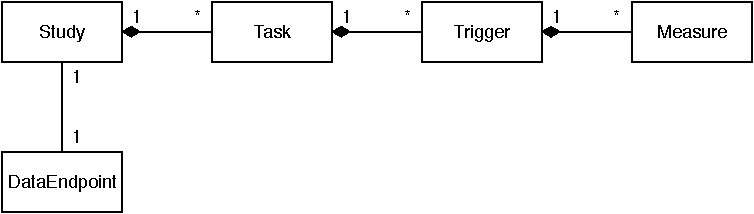
\includegraphics[width=0.8\textwidth]{images/CAMS-UML.pdf}
    \caption{A UML diagram of the \textit{CAMS} Domain Model.}
    \label{fig:cams_uml}
\end{figure}

Concretely, a \textit{Study} holds a set of \textit{Triggers}, which define \textit{when} sampling is carried out, such as by scheduling sampling at  given time each day, or when a certain event is registered, such as entering a specific \textit{GeoFence}\footnote{\url{https://developers.google.com/location-context/geofencing}}. 

Each \textit{Trigger} holds one or more \textit{Tasks}, each of which define which \textit{Measures} should run simultaneously. In addition, a \textit{Task} also defines whether or not data is sampled in the background, or whether the user needs to interact with the device in order to perform sampling. 

Each \textit{Task} holds a set of \textit{Measures} each of which defines what to sample, i.e. which data channel to listen to. Lastly, a \textit{Study} also holds a reference to the \textit{DataEndpoint} specifying which where data ends up, i.e. by uploading it to a server.

An integration for the CAMS Framework will be described later in this thesis. 


% 1 Show you know the literature
% there is far too much literature for you to be exhaustive, so you must be selective
% 2 Gives your readers background to understand your work
% this includes both readers who are specialists in your area, and readers who know nothing about it (e.g., external examiners). Its a delicate balancing act
% 3 Gives a historical perspective
% shows how ideas arose and evolved over time
% 4 Leads into the problem you wish to tackle in your thesis
% what others have done before within this context, what is being done now, what problems have been identified, what has not been worked on, how your own work builds / adds onto this
% 5 Describes related work
% illustrates other ideas related to your research idea i.e., how they are in common and how they are different
% explains why your idea or perspective is new
% 6 Gives a new view of the problem / solution space
% 7 Synthesis: combines together the literature in a way that adds something new i.e., the whole is greater than the sum of the parts
% birds eye view: as a reader of the literature, you now have a better perspective than any individual author may have had (particularly earlier authors who have not seen later work). You can now 'step back' and give a coherent overview of all that has happened
% framework: fits all the pieces together into an organization that relates all the parts
